\subsection{\eigenfaces{}}\label{subsec:eigenface}

According to \citeauthor{eigenfaces1991}, the idea of \eigenfaces{} is inspired by information theory.
Opposed to former approaches in the domain of face recognition which relied on the classification of images based on a set of predefined facial features, 
such as distance between eyes,
\eigenfaces{} does not use predefined features \cite{eigenfaces1991}.
The goal of this approach is to represent images using a smaller set of image features, i.e.\ compression to a lower-dimensional feature space, 
such that it is possible to distinguish between the images \cite{eigenfaces1991, eigenfaces2013}.
These features do not necessarily correspond to human facial features \cite{eigenfaces1991}.
Similar pictures, i.e.\ of the same person, should lie on a manifold in the lower-dimensional feature space \cite{face-recognition2008}.
The decomposition of input images not only reduces the complexity but also facilitates modeling probability density of a face image \cite{face-recognition2008}.

% input image
% greyscale
The greyscale input images are two-dimensional arrays of numbers: $\textbf{x} = \left\{ x_i \vert i \in \textbf{S} \right\}$, $\textbf{S}$ being a square lattice \cite{eigenfaces1997, eigenfaces1991}.
The images are reshaped to an one-dimensional array $\textbf{x} = \left[x_1, x_2, ..., x_n  \right]^{T} \in \mathbb{R}^{n}$, 
where $n = \left\| \textbf{S} \right\|$ and $\mathbb{R}^{n}$ is the $n$-dimensional euclidean space \cite{eigenfaces1997}.
% background
Some authors stress that the background is removed to omit values outside the face area \cite{eigenfaces1991}.
% dimension
In literature, typically, the original images' dimension is 512x512 \cite{eigenfaces1991} or 64x64 \cite{face-recognition2020}, 
whereas the projected images' dimension is 16x16 \cite{eigenfaces1991} or 250 \cite{face-recognition2020} respectively.
% normalization/ centering
\citeauthor{eigenfaces1991} stress that the data should be normalized, i.e.\ centered: 
$\Phi_{k} = \mathbf{x}_{k} - {\psi }$. 
$\Phi_{k}$ being the difference of the $k$-th training image and the average image $\psi = \frac{1}{N}\sum_{k=1}^{N}\textbf{x}_{k}$, $N$ being the number of training images.

% decomposition
The next step is to find an alternative lower-dimensional representation of the images, which preserves most of the information of the original image.
In mathematical terms, this decomposition can be expressed as 
$\textbf{x} = \sum_{i=1}^{n}\hat{x}_{i} \textbf{e}_{i}$, 
%$\hat{x}_{i}$ being inner product of $\textbf{x}$ and $\textbf{e}_{i}$,
$\textbf{e}$ being an orthogonal basis 
\cite{eigenfaces1997}.
If all basis vectors are used, the original image can be reconstructed using a linear combination of the basis vectors \cite{eigenfaces1991, face-recognition2020}.
The number of basis vectors is limited by the minimum of the training set size $N$ \cite{eigenfaces1991} and the number of pixels $n$ \cite{face-recognition2020}.
In order to compress the input from a $n$ to a $m$-dimensional space, given $m \ll n$, only the first $m$ basis vectors are used.
The parameter $m$ and the basis $\textbf{e}$ is chosen such that $\hat{x}_{i}$ is small for $i \ge m$ \cite{eigenfaces1997}.
The compressed version of the image is denoted $\textbf{x} \simeq \hat{\textbf{x}} = \left[\hat{x}_{1}, \hat{x}_{2}, ..., \hat{x}_{m}  \right]^{T}$.
In other words: 
The compressed image is a vector of the first $m$ weights of the linear combination of weight and basis vectors used to transform the compressed image back to the original space.
The weights denote the position of the projection of the face images in the feature space or so-called face space spanned by the first $m$ basis vectors \cite{eigenfaces1991}.

% eigenfaces: KL base
In the context of \eigenfaces{}, one basis used for decomposition is the \ac{kl} basis, i.e.\ \ac{pca} \cite{eigenfaces1997, eigenfaces1991}.
% source 1991, pg. 587: or fourier basis
According to \citeauthor{eigenfaces1997}, the \ac{kl} representation is optimal in the sense that it minimizes the \ac{rmse} between the original image and 
the compressed image calculated using $m < n$ orthogonal vectors.
The \ac{kl} basis consists of the eigenvectors of covariance matrix $\textbf{C} = E\left[ \textbf{x}\textbf{x}^{T} \right]$ of the input images $\mathbf{x}$ \cite{eigenfaces1997}.
% determine the number of components m
Since these eigenvectors can have facial features, they are called \textit{\eigenfaces{}}.
There are two approaches in the literature to determine the number of \eigenfaces{} $m$ used to compress the input images:
\begin{enumerate}[label=(\alph*)]
    \item The cumulative explained variance of the first $i \le n$ eigenvectors (sorted by eigenvalues $\lambda_i$) is calculated 
        \cite{eigenfaces1997, face-recognition2020, face-recognition2021}.
        The eigenvalues $\lambda_i$ can be interpreted as the amount of variance explained by the corresponding eigenvector $\textbf{e}_i$, which is equivalent to information or entropy.
        The user can choose how much variance, i.e.\ information, should be preserved, by choosing $m$ such that the explained variance is greater than a chosen threshold.
        \citeauthor{face-recognition2021} use a threshold of 90\%.
        A plot displaying the cumulative explained variance and a threshold of 90\% is shown in \autoref{fig:det_n_comp} (a).

    \item The number of \eigenfaces{} $m$ is chosen using the reconstruction error-complexity trade-off. % \cite{face-recognition2008}.
        The reconstruction error, i.e.\ the \ac{rmse} of the original image $X$ and the inverse transformed image $X'$, is 
        calculated in \autoref{eq:rsme} for different values of $m$.
        The "elbow" point marks the point where the reconstruction error decreases only slightly for increasing $m$ and thus, is an indicator for the optimal $m$.
        A visualization of this approach is shown in \autoref{fig:det_n_comp} (b).
\end{enumerate}

\begin{equation}
    \text{RSME} = \sqrt{\frac{\sum_{i=1}^{N}(x_{i}-x'_i)^2}{N}}
    \label{eq:rsme}
\end{equation}
 
\begin{figure}%
    \centering
    \subfloat[\centering The cumulative explained variance of the first $i \le n$ eigenvectors (sorted by eigenvalues $\lambda_i$).]
    {{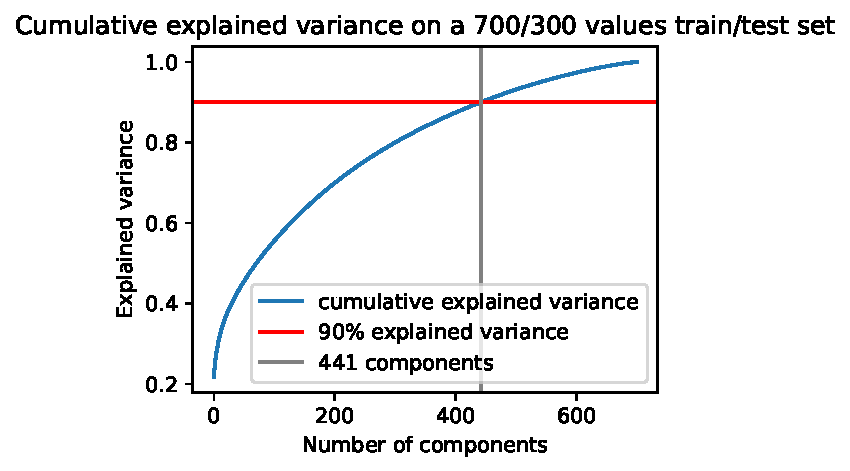
\includegraphics[width=7cm]{images/Eigendocs/Eval-Params/cumulative_explained_variance.pdf}}}%
    \qquad
    \subfloat[\centering The reconstruction error \ac{rmse} calculated for different values of $m$. 
    The reconstruction error increases less rapidly after 10 to 20 components.]
    {{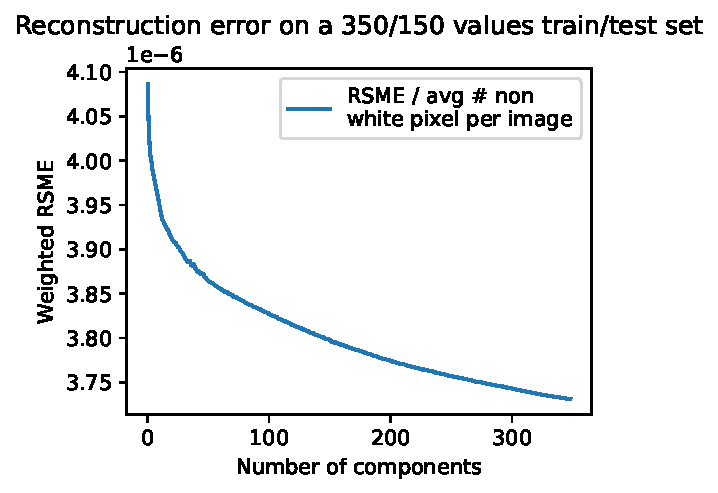
\includegraphics[width=7cm]{images/Eigendocs/Eval-Params/pca_reconstruction_error.pdf} }}%
    \caption[Approaches to find the number of \eigenfaces{}]{Two approaches to determine the number of \eigenfaces{} $m$ used to compress the input images.}%
    \label{fig:det_n_comp}%
\end{figure}

% calculation of eigenvectors of covariance matrix C
In order to reduce calculation complexity, $C$ is approximated.
% 1997
\citeauthor{eigenfaces1997} propose the approximation $\textbf{C} \simeq \frac{1}{N}\sum_{k=1}^{N}\textbf{x}_{k}\textbf{x}_{k}^{T} = \frac{1}{N}\textbf{X}\textbf{X}^{T}$, 
with $\textbf{X} = \left[ \textbf{x}_{1}, \textbf{x}_{2}, ..., \textbf{x}_{N} \right]$, $\textbf{x}_i \in \mathbb{R}^{n}$ \cite{eigenfaces1997}.

Finding the eigenvectors of $\textbf{X}\textbf{X}^{T}$ is still computationally expensive, since $\textbf{X}\textbf{X}^{T}$ is a $n$ by $n$ matrix.
According to \citeauthor{eigenfaces1997}, the eigenvectors of $\textbf{X}\textbf{X}^{T}$ can be calculated by using the eigenvectors of $\textbf{X}^{T}\textbf{X}$.
The eigenvectors $\textbf{e}_i \in \mathbb{R}^{n}$ of $\textbf{X}\textbf{X}^{T}$ can be derived from the eigenvectors $\textbf{v}_i \in \mathbb{R}^{N}$ of $\textbf{X}^{T}\textbf{X}$ by 
$\textbf{e}_i = \frac{1}{\sqrt{\lambda_i}}\textbf{X}\textbf{v}_i$ as discussed in more detail in \cite{eigenfaces1997}.
According to \citeauthor{dim_reduction2021}, the problem is reduced to a $N$ by $N$ matrix, which is computationally less expensive to solve assuming $N \ll n$.
Eigenvectors can be calculated using \ac{svd} \cite{eigenfaces1997}.
\ac{svd} is a method, which decomposes a matrix into the so-called left singular vector, the diagonal matrix and the right singular vector \cite{dim_reduction2021}. 

% classification/ compare
In the literature, face images are classified by comparing their position in the face space with those of already known faces \cite{eigenfaces1991}.
% performance 
According to \cite{eigenfaces1991}, this approach performs well on datasets with little variation in pose, lighting and facial expression.
However, \Citeauthor{eigenfaces1997} state, that the performance deteriorates if the variations increase since the changes introduce a bias 
and thus, the distance function used to make classifications is no longer a reliable measure.